% Объединение возможностеи
\label{collective_global}

%\todo[inline]{Надо применить единообразный стиль функций, либо все с ($\cdot$), либо все без ($\cdot$).}

Если оценку параметров объектов $x_{ij}$ для задачи выбора объектов (см. раздел~\ref{selection_task}) совершают несколько экспертов, исходным материалом для программного комплекса служит набор экспертных оценок $\{\p^{(r)}_{ij}(\cdot)\}$ --- распределений нечётких элементов $\tilde x_{ij}$, где $r = \dotR$ --- номер эксперта, $i = \dotN$ --- номер объекта, $j = \dotM$ --- номер параметра объекта.

На вход алгоритма выбора объектов подаётся только набор оценок $\{\p_{ij}(\cdot)\}$, $i = \dotN$, $j = \dotM$, выражающий мнение одного эксперта или коллективное мнение экспертов (см. рис.~\ref{ris:program_global}), поэтому в настоящем разделе ставится задача сведения набора $\{\p^{(r)}_{ij}(\cdot)\}$ к набору $\{\p_{ij}(\cdot)\}$ --- задача нахождения  оценок, выражающих коллективное мнение экспертов, или, короче говоря, задачи <<коллективной экспертизы>>. 

\begin{figure}[h]
\center{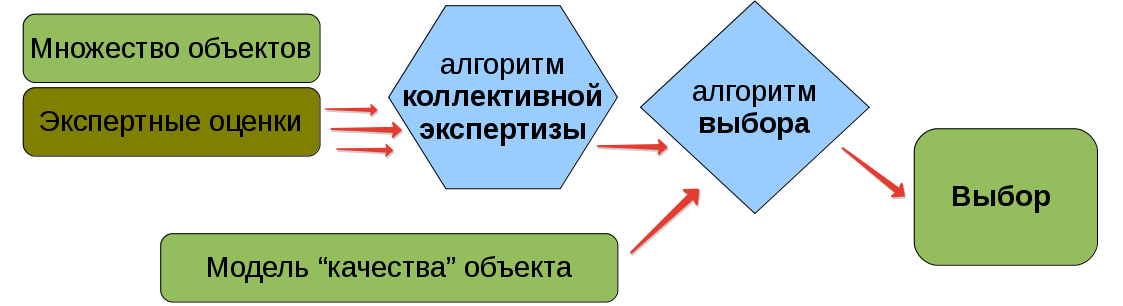
\includegraphics[width=0.85\linewidth]{./pic/globalscheme}}  
\caption{\small Схема, иллюстрирующая работу программного комплекса в режиме нахождения наиболее <<качественных>> объектов на выходе по мнениям нескольких экспертов и модели <<качества>> объектов (функции $f$, см. \eqref{e:function_f} на стр. \pageref{e:function_f}).}
\label{ris:program_global}
\end{figure}

Задача коллективной экспертизы в рамках использования модели нечётких оценок в теории возможностей Пытьева может быть поставлена и решена различными методами. Рассмотрим два класса:
	\begin{enumerate}
		\item Методы, в рамках которых экспертные оценки, выраженные распределениями возможности, рассматриваются как элементы метрического пространства, а задача коллективной экспертизы ставится как задача поиска оценки, наиболее близкой в среднем квадратичном к множеству распределений, заданных разными экспертами  \cite{pytyev_experts}: метод матриц попарных сравнений, векторов предпочтений, векторов перестановок и др.;
		\item Новый метод, в рамках которого экспертные оценки рассматриваются как элементы полурешётки 
		--- частично упорядоченного множества, для каждой пары элементов которого в этом множестве найдётся точная верхняя  грань (супремум), % см. раздел~\ref{easy_collective_sup}, 
		а задача коллективной экспертизы ставится как задача поиска оценки, являющейся верхней гранью множества оценок, заданных разными экспертами.
	\end{enumerate} 
	

%=========================	
\subsection{Поиск оценки, близкой в среднем квадратичном к оценкам различных экспертов}
\label{easy_collective_matrix_vector}

Теоретико-возможностная модель всех параметров всех объектов в задаче выбора определяется распределением $\p(\cdot):\ X\to[0,1]$ нечёткого вектора $\theta = \tetavector$, заданным формулой~\ref{e:p_theta_def}. Пусть из разных источников (от разных экспертов) получена информация, выраженная распределениями 
\begin{equation}
\label{pr_theta_def}
	\p_r(\cdot): T \rightarrow \zo,\; \p_r \big(\tvector\big) =  \inf_{\substack{i \in \setN \\ j \in \setM}}\,\p^{(r)}_{ij}(x_{ij}), 
\end{equation}
где $r = \dotR$ --- номер эксперта, и на основе этой информации должно быть построено неизвестное распределение $\p(\cdot)$, являющееся коллективным мнением экспертов по отношению к экспертным мнениям $\p_r(\cdot)$. 

%\subsubsection{Общий принцип}
%\label{euclidean_basics}

Поскольку каждая экспертная оценка из набора $\{\p_r(\cdot) \,|\, r = 1, \ldots, R\}$ задана в своей субъективной шкале (в которой работает $r$-й эксперт), то сравнивать между собой числовые значения возможностей в оценках от разных экспертов нельзя. Однако можно построить максимальный инвариант группы $\bTheta$, введённой в разделе~\ref{sec:sec_20151029_02}, как функцию возможностных распределений. Пусть множество $\calM$ --- область значений максимального инварианта. 

Элементы $\calM$, как и возможностные распределения, есть экспертные мнения, и можно найти элементы $\calm_r \in \calM$, эквивалентные экспертным оценкам $\p_r(\cdot)$, $r = 1, \ldots, R$. Численное значение $\calm_r$ можно содержательно интерпретировать, поскольку оно не изменится при переходе от одного породающего  $\calm_r$ распределения $\p_r(\cdot)$ к другому, эквивалентному ему распределению $\gamma(\p_r(\cdot)),\, \gamma \in \bTheta$. На множестве $\calM$ можно ввести метрику $\rho(\calm, \calm')$, где $\calm, \calm' \in \calM$.

%Методы <<евклидовой близости к среднему>> заключаются в поиске элемента, сумма евклидовых расстояний до которого от мнений отдельных экспертов была бы минимальной. Известно, что такая постановка задачи приводит к поиску среднего арифметического экспертных мнений (которое само по себе может не являться элементом $\calM$), а затем поиску максимально близкого в евклидовой метрике к этому среднему арифметическому элемента из $\calM$.  

Следуя логике~\cite{pytyev_experts}, дополним множество $T$ размера $\abs{T}$ ещё одним вектором $t_{\abs{T}+1}$, получив множство $T^+$, и положим $\p^{(r)}(t_{\abs{T}+1}) \define= 0$. Возможностное распределение $\p(\cdot): T^+ \to\zo$\footnote{Обозначения $\p(\cdot)$ и подобные ему сохраним без изменений, далее \emph{в этом разделе} везде имея в виду по умолчанию $\p(\cdot): T^+ \to\zo$.} конструктивно получается из $\p(\cdot): T^+ \to\zo$ добавлением нуля и, таким образом, всегда содержит точку с возможностью нуль. Это сделано для того, чтобы при переходе от множества возможностных распределений к множеству $\calM$ и обратно не потерять точки, где возможность равна нулю, играющие особую роль в теории возможностей.

\subsubsection{Метод матриц попарных сравнений}
\label{easy_collective_matrix}
Пусть множество $T^+$ конечно. Пронумеруем все векторы $t \in T^+$ индексами, принимающими значения от $1$ до $\abs{T^+}$.
Тогда $T^+ = \{t_1, \mydots, t_{\abs{T^+}}\}$. Матрицы попарных сравнений определяются покоординатно через экспертные оценки $\p_{r}(\cdot): T^+ \to\zo$, $r = \dotR$:
      \begin{gather}
      \label{matrixM_def}
	   m^{(r)}_{kj} = \begin{cases}
		\;\;\;1,\;\; \p_{r}(t_k) > \p_{r}(t_j),\\
		\;\;\;0,\;\; \p_{r}(t_k) = \p_{r}(t_j),\\
		-1, \;\; \p_{r}(t_k) < \p_{r}(t_j),
	  \end{cases} 
	   k,j = 1\ldots\abs{T^+}.  
      \end{gather}

Не всякая матрица нужного размера с элементами $0, 1, -1$ является матрицей попарных сравнений. Матрица попарных сравнений должна быть антисимметрична, а также удовлетворять следующему условию, выражающему транзитивность отношений <<$=$>>, <<$<$>> и <<$>$>>:
\begin{equation}
\label{transitive_matrix}
    m_{ij} = m_{jk} = a \Rightarrow m_{ik} = a,  \text{где }  i,j,k = 1\ldots\abs{T^+}.
\end{equation}  
	Множество $M$ матриц $m$, определённых с помощью~\eqref{matrixM_def},\eqref{transitive_matrix} и антисимметричных, есть частный случай множества $\calM$, о котором говорилось в разделе~\ref{euclidean_basics}.

Задача коллективной экспертизы как задача поиска матрицы попарных сравнений $m_*$, выражающей коллективное мнение экспертов, ставится так:	      
      \begin{gather}
      \label{zad_matrix}
	  m_* = \arg \min_m \sum_{r=1}^{R} \rho(m^{(r)}, m),
	  \text{где } \rho(m, m') = \big( \sum_{k,j=1}^{\abs{T^+}}(m_{kj} - {m'}_{kj})^2 \big)^{1/2}.
      \end{gather}

Из-за требования~\eqref{transitive_matrix} $m_*$ не всегда легко найти, и в настоящее время нет алгоритма, которой бы  решал задачу~\eqref{zad_matrix} для любых входных данных. 

\subsubsection{Метод векторов предпочтений}
\label{easy_collective_vector}
Пусть множество $T^+$ конечно. Пронумеруем все векторы $t \in T^+$ индексами, принимающими значения от $1$ до $\abs{T^+}$.
Тогда $T^+ = \{t_1, \mydots, t_{\abs{T^+}}\}$.  Векторы предпочтений определяются покоординатно через экспертные оценки $\p_{r}(\cdot): T^+ \to\zo$, $r = \dotR$:
	\begin{gather}
	 \label{vectorS_def}
		s^{(r)}_j = \sum_{t \in T} {\mathlarger{\chi} }_{A^{(r)}_j(t)},  j \in J. \\ 
		 \text{Здесь } A^{(r)}_j = \{t \in T: \p_{r}(t) \leq \p_{r}(t_j)\}, 
		 \\ {\mathlarger{\chi}}_A(\cdot)  \text{--- индикатриса множества $A$.}
	 \end{gather}


	Разумеется, не всякий вектор нужного размера есть вектор предпочтений. Вектор предпочтений $s$ должен удовлетворять условию:
	%\\ (1) $\max s_j= |T|$ (нормировка возможности);
	\begin{equation}
	    \label{vectorS_cond}
	    |J_i| = i, \text{где } J_i = \{j \in J: s_j \leq i\}, i \in \{s_1 \ldots s_{\abs{T^+}}\}.
	\end{equation} 
	Множество $S$ векторов $s$, определённых с помощью~\eqref{vectorS_def} и~\eqref{vectorS_cond}, есть частный случай множества $\calM$, о котором говорилось в разделе~\ref{euclidean_basics}.
	
	Задача коллективной экспертизы как задача поиска вектора предпочтений $s_*$, выражающего коллективное мнение экспертов, ставится так:	    		
	\begin{equation}
	\label{zad_vectorS}
	      s_* = \arg \underset{s} \min \sum_{r=1}^R \rho(s - s^{(r)}), \text{где }  \rho(s, s') = \big( \sum_{j=1}^{\abs{T^+}}(s_{j} - {s'}_{j})^2 \big)^{1/2}.
	\end{equation} 
	
	Алгоритм решения этой задачи такой: берём  вектор $ \ol s =  \frac{1}{R} \sum_{r=1}^R s^{(r)}$ и удовлетворяем условию~\eqref{vectorS_cond} с помощью округления и (если требуется) дополнительного изменения его координат. На ЭВМ такое дополнительное изменение координат можно производить итеративно: за одну итерацию некоторые координаты изменяются на одну единицу, после чего производится проверка условия~\eqref{vectorS_cond} и так далее, пока не будет найдет элемент $s \in S$.  %Такой алгоритм, сходящийся к элементу $s \in S$, был реализован в ходе работы. %На многих входных данных он даёт решение задачи~\eqref{zad_vectorS}.   

%=========================
\subsection{Вычисления супремума множества экспертных оценок}
\label{easy_collective_sup}

\subsubsection{Квазипорядок на множестве возможностных распределений}
\label{preorder_pyt}

Определение квазипорядка на множестве $U$ аналогично определению порядка \eqref{interv_order}, за исключением отсутствия требования равенства в качестве эквивалентности~\cite{Mirkin}:  
 \begin{equation}
\label{preoder_def}
\begin{split}
\forall A \in U: & A \prec A; \\
\forall A, B, C \in U: & A \prec B \text{ и } B \prec C \Rightarrow A \prec C.
\end{split}
\end{equation}

На множестве возможностных распределений, определённых на (одном и том же, фиксированном) множестве $X$, то есть на множестве функций\footnote{В этом и нескольких следующих пунктах повествования, отвелкаясь от задачи выбора объектов, используются обозначения $\p(\cdot), \p_1(\cdot), \p_2(\cdot): X\to \zo$. Переход повествования обратно к $\p_{ij}(\cdot),\p_{ij}^{(r)}(\cdot): X\to \zo $ и $\p(\cdot),\p_{r}(\cdot): T\to \zo $ будет явно указан.} $\p(\cdot):\ X\to[0,1]$, таких что $\displaystyle \sup_{x\in X} \p(x) = 1$, введём отношение~<<$\prec$>>: $\p_1\prec\p_2$, если:
\begin{enumerate}
    \item\label{order-D1}
        носитель $\p_1(\cdot)$ меньше (по включению), чем носитель $\p_2(\cdot)$: $\supp\,\p_1\subset\supp\,\p_2$;
    \item\label{order-D2}
        найдётся непрерывная монотонная функция ${\mygamma(\cdot):\ [0,1]\to[0,1]}$, $\mygamma(0) = 0$, $\mygamma(1) = 1$, такая что $\p_2(x) = \mygamma(\p_1(x))$ при $x\in\supp\,\p_1$;
    \item\label{order-D3}
        значения распределения $\p_2(\cdot)$ на носителе распределения $\p_1(\cdot)$ не меньше, чем значения $\p_2(\cdot)$ вне носителя $\p_1(\cdot)$:
        $$\inf\{\p_2(x) \mid x\in\supp\,\p_1\} \geqs \sup\{\p_2(x) \mid x\in X\setminus\supp\,\p_1\};$$
\end{enumerate}
где $\supp\, \p_i = \{x\in X:\ \p_i(x) > 0\}$~--- носитель распределения $\p_i(\cdot),\ i=1,\, 2$.

Можно показать, что отношение <<$\prec$>> является отношением квазипорядка, то есть рефлексивно и транзитивно. При этом из $\p_1\prec\p_2$ и $\p_2\prec\p_1$ не следует тождественное равенство $\p_1(\cdot)$ и $\p_2(\cdot)$, однако из этого следует эквивалентность возможностных распределений $\p_1(\cdot)$ и $\p_2(\cdot)$, то есть существование непрерывной строго монотонной функции $\gamma (\cdot):\ [0,1]\to[0,1]$, $\gamma(0) = 0$, $\gamma(1) = 1$, такой что $\p_2(x) = \gamma(\p_1(x))$ при $x\in X$ (см. принцип относительности возможностей~\ref{sec:sec_20151029_02}).

В случае, если распределения $\p_1(\cdot)$ и $\p_2(\cdot)$ сравнимы, то есть $\p_1\prec\p_2$ или $\p_2\prec\p_1$, будем говорить, что эти распределения не противоречат друг другу, а запись $\p_1\prec\p_2$ будем читать как <<$\p_1$ уточняет $\p_2$>>. Это связано с интерпретацией квазипорядка <<$\prec$>> как отношения, упорядочивающего возможностные распределения по степени их \emph{информативности}. Такая интерпретация может быть проиллюстрирована тем, что всякое распределение, достигающее значения 1 в некоторой точке $x_0 \in X$, уточняет тривиальное распределение, тождественно равное 1, и одновременно с этим уточняется <<$\delta$-образным>> распределением, принимающим значение 1 в точке $x_0$ и значение 0 во всех остальных точках $X$ (см. рис.~\ref{ris:half_lattice}).

\subsubsection{Содержательная интерпретация квазипорядка на множестве возможностных распределений}
\label{preorder_explain}

Обоснование содержательной интерпретации отношения <<$\prec$>> основано на его роли в следующей задаче принятия решений.

Пусть $\eta$ и $\zeta$~--- нечёткие элементы со значениями в $Y$ и $Z$ соответственно, совместное распределение возможностей которых есть $\p(\cdot):\ Y\times Z\to[0,1]$, и по реализации $y\in Y$ элемента $\eta$ требуется принять решение о реализации $z\in Z$ элемента $\zeta$. Множество чётких стратегий, минимизирующих возможность ошибки при $\p(\cdot) = \p_1(\cdot)$, обозначим $D_1$, при $\p(\cdot) = \p_2(\cdot)$~--- $D_2$.
Имеет место следующая теорема.

\begin{theorem}
\label{theorem_zubyuk}
    Пусть $\p_1\prec\p_2$, и множества $D_1$ и $D_2$ не пусты. Тогда при $\p(\cdot) = \p_1(\cdot)$ всем стратегиям из $D_1$ соответствует либо ненулевая возможность ошибки, при этом $D_1\subset D_2$, либо нулевая возможность ошибки, при этом для всякой $d_1\in D_1\setminus D_2$ найдётся такая стратегия $d_1'\in  D_1\cap D_2$, что возможность несовпадения решений, принятых с использованием $d_1$ и $d_1'$, равна нулю.
\end{theorem}

%Рассмотрим подробно смысл данной теоремы.
Итак, если всякой стратегии из множества $D_1$ соответствует ненулевая возможность ошибки, то $D_1\subset D_2$, то есть использование распределения $\p_1(\cdot)$ вместо $\p_2(\cdot)$ позволяет сузить множество оптимальных стратегий. 
Это согласуется со следующей трактовкой отношения <<$\prec$>>: 
\begin{center} \fbox{ 
\begin{minipage}{0.9 \textwidth}
 $\p_1\prec \p_2 \Leftrightarrow$ распределение $\p_1(\cdot)$ не менее информативно, чем $\p_2(\cdot)$. Чем более информативно распределение, тем более конкретный ответ (более узкое множество оптимальных стратегий) оно позволяет получить в задаче принятия решений.
 \end{minipage}
} \end{center}

%В случае, если всем стратегиям из множества $D_1$ соответствует нулевая возможность ошибки, множество $D_1$, вообще говоря, не уже, чем множество $D_2$. Однако для всякой стратегии $d_1\in D_1\setminus D_2$ в этом случае найдётся эквивалентная ей стратегия $d_1'\in D_1\cap D_2$; эквивалентность здесь понимается как равенство нулю возможности несовпадения принятых с использованием $d_1$ и $d_1'$ решений при $\p(\cdot) = \p_1(\cdot)$.

%Таким образом, пополнение множества оптимальных стратегий при использовании распределения $\p_1(\cdot)$ вместо $\p_2(\cdot)$ может быть связано исключительно с тем, что некоторые элементарные исходы, имеющие ненулевую возможность при $\p(\cdot) = \p_2(\cdot)$, имеют нулевую возможность при $\p(\cdot) = \p_1(\cdot)$. Только при реализации таких исходов эквивалентные стратегии из множеств $D_1\setminus D_2$ и $D_1\cap D_2$ приводят к принятию разных решений.

%Однако, тот факт, что некоторые элементарные исходы, имеющие ненулевую возможность при $\p(\cdot) = \p_2(\cdot)$, имеют нулевую возможность при $\p(\cdot) = \p_1(\cdot)$, как раз и означает, что распределение $\p_1(\cdot)$ более информативно, чем $\p_2(\cdot)$: распределение $\p_1(\cdot)$ более конкретно, более чётко определяет исход эксперимента, так как множество возможных исходов при $\p(\cdot) = \p_1(\cdot)$ уже, чем при $\p(\cdot) = \p_2(\cdot)$.	
	
\subsubsection{Супремум и инфинум возможностных распределений}
\label{inf_sup_poss}

Пользуясь введённым в разделе~\ref{preorder_pyt} отношением квазипорядка, для любой пары распределений $\p_1(\cdot)$ и $\p_2(\cdot)$ распределение $\p_1\vee\p_2(\cdot)$ определим как их супремум (если он существует), то есть как наиболее информативное среди всех распределений, уточняемых обоими распределениями $\p_1(\cdot)$ и $\p_2(\cdot)$. Распределение $\p_1\wedge\p_2(\cdot)$ определим как инфимум $\p_1(\cdot)$ и $\p_2(\cdot)$ (если он существует), то есть как наименее информативное среди всех распределений, уточняющих $\p_1(\cdot)$ и $\p_2(\cdot)$.

Можно показать, что в случае, если область определения возможностных распределений конечна, супремум существует для любой пары распределений.  Тогда множество всех распределений образует полурешётку с идемпотентной, коммутативной и ассоциативной алгебраической операцией <<$\vee$>>, см. рис.~\ref{ris:half_lattice}. 
\begin{notice}
В случае, если область определения возможностных распределений конечна, инфимум тоже существует для любой пары распределений, если множество всех распределений пополнено функцией $0(\cdot)$, тождественно равной нулю на всей области определения (заметим, что с формальной точки зрения такая функция не является возможностным распределением, так как не найдётся точки, возможность которой равна 1). Более того, можно показать, что какой бы ни была область определения возможностных распределений, пополнение множества распределений функцией $0(\cdot)$ является необходимым условием существования инфимума для любой пары распределений. Если для любой пары возможностных распределений существуют и супремум и инфимум, множество всех распределений, пополненное $0(\cdot)$, образует решётку с алгебраическими операциями <<$\vee$>> и <<$\wedge$>>, являющимися идемпотентными, коммутативными и ассоциативными.
\end{notice}
%Lalaa $\mathlarger{ \succ }$.

\begin{figure}[h]
\center{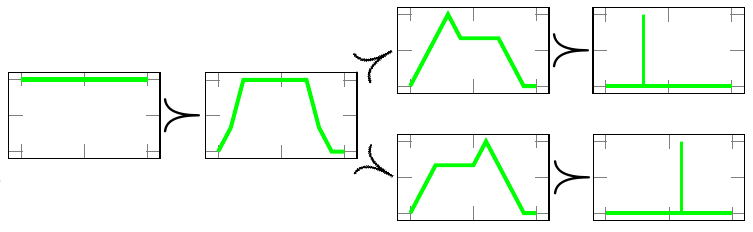
\includegraphics[width=0.9\linewidth]{./pic/lattice3}}  
\caption{\small Полурешётка возможностных распределений. Справа --- <<$\delta$-образные>> распределения, уточняющие распределения с точками единичной возможности в тех же местах (левее). Ещё левее --- супремум верхнего и нижнего распределений. Слева --- тривиальное распределение, которое уточняется всеми остальными. }
\label{ris:half_lattice}
\end{figure}

\subsubsection{Численный алгоритм вычисления супремума}
\label{algo_sup_poss}

Доказана система теорем, позволившая разработать численный метод построения супремума возможностных распределений и его компьютерную реализацию. Алгоритм построения $\p_1 \vee\p_2(\cdot)$ в случае конечной области определения $X$ возможностных распределений $\p_1(\cdot), \p_2(\cdot)$ (когда супремум всегда существует) выглядит следующим образом.
\begin{enumerate}
	\item 
		Если $\supp\,\p_1(\cdot) = \supp\,\p_2(\cdot) = X_s \subset X$, то и $\supp \; \p_1 \vee\p_2(\cdot) = X_s$. При этом, если упорядоченность элементарных событий по возможности в распределениях $\p_1(\cdot)$ и $\p_2(\cdot)$ одинакова, то есть: 
		\begin{equation*}
		%	\label{non_contradict_p1p2}
			\forall\, x_1, x_2 \in X_s: \p_1(x_1) \geq \p_1(x_2) \Rightarrow  \p_2(x_1) \geq \p_2(x_2), 
		\end{equation*}
		то можно в качестве супремума взять, например, $\p_1(\cdot)$ или $\p_2(\cdot)$. Поэтому алгоритм в случае совпадающих носителей устроен так:
		\begin{enumerate}
		    \item 
		    В качестве начального приближения, для определённости, положим $\p_1 \vee\p_2(\cdot) = \p_1(\cdot)$.
		    \item
		    Для всех таких точек $x_1, x_2 \in X_s$, для которых выполняется
		    \begin{equation}
			\label{contradict_p1p2}
			  \p_1(x_1) \geq \p_1(x_2) \text{, но } \p_2(x_1) \leq \p_2(x_2), 
		     \end{equation}		    
		     находим <<промежуточные>> точки  
		    \begin{equation*}
			X_w = \{x:  \p_1(x_2) \leq \p_1(x) \leq \p_1(x_1)\} \bigcup \{x:  \p_2(x_1) \leq \p_2(x) \leq \p_2(x_2)\}.
		    \end{equation*}		    
		    Во всех точках $x \in X_w$ из-за условия~\eqref{contradict_p1p2} следует положить одинаковые значения функции $\p_1 \vee\p_2(\cdot)$. Например, полагаем
		    \begin{equation*}
			\p_1 \vee\p_2(x) = \sup_{x' \in X_w} \p_1(x'),\, x \in X_w.
		    \end{equation*}	
		\end{enumerate}   
		%Все остальные случаи сводятся к этому.
	\item 
		Если $\supp\,\p_1(\cdot) \subset \supp\,\p_2(\cdot)$, необходимо заменить $\p_1(\cdot)$ на $\tilde \p_1(\cdot)$ таким образом, что $\p_1 \vee\p_2(\cdot) = \tilde \p_1 \vee\p_2(\cdot)$  но уже $\supp\,\tilde \p_1(\cdot) = \supp\,\p_2(\cdot)$, что вернёт нас к случаю (1). Это делается, например, так:
		\begin{equation*}
			\tilde \p_1(x) = \begin{dcases}
						\p_1(x), & x \in \supp\,\p_1;
						\\ \p_2(x)\frac{\displaystyle \inf_{ x' \in \supp\,\p_1(\cdot)}\, \p_1(x')}{\displaystyle 2 \sup_{ x' \in \supp\,\p_2(\cdot) \setminus \supp\,\p_1(\cdot)}\, \p_2(x')}, & x \in \supp\,\p_2(\cdot) \setminus \supp\,\p_1(\cdot);
						\\ 0, & x \in X \setminus \supp\,\p_2(\cdot).
						\end{dcases}			
		\end{equation*}
	\item 
	  Если $\supp\,\p_2(\cdot) \subset \supp\,\p_1(\cdot)$, замена $\p_1(\cdot) \leftrightarrow \p_2(\cdot)$ сводит этот случай к случаю (2).
	\item
	  Если $\supp\,\p_1(\cdot) \setminus \supp\,\p_2(\cdot) \neq \varnothing$  и  $\supp\,\p_2(\cdot) \setminus \supp\,\p_1(\cdot) \neq \varnothing$, необходимо заменить $\p_1(\cdot)$ \emph{и} $\p_2(\cdot)$ на $\tilde \p_1(\cdot), \tilde \p_2(\cdot)$ таким образом, что $\p_1 \vee\p_2(\cdot) = \tilde \p_1 \vee \tilde \p_2(\cdot)$,  но уже $\supp\,\tilde \p_1(	\cdot) = \supp\,\tilde \p_2(\cdot)$, что вернёт нас к случаю (1). Это делается, например, так: 
	 % \begin{comment}
	  \begin{equation*}
	  \begin{split}
			\text{Пусть везде }  &i,j=1,2,\, i\neq j; \\
			\text{Пусть }  &\ubar{\p}_i = \inf_{ x' \in \supp\,\p_i(\cdot)}\, \p_i(x'); \\
			\text{Пусть }  &\obar{\p}_i = \sup_{ x' \in \supp\,\p_i(\cdot)\setminus \supp\,\p_j(\cdot)}\, \p_i(x');\\	
			\text{Пусть }  &\mygamma(y) = \begin{dcases}
										  y\frac{\obar{\p}_i}{\ubar{\p}_i}, & y \in [0,\,\ubar{\p}_i];
										 \\  \obar{\p}_i, & y \in [\ubar{\p}_i\,\obar{\p}_i];
										  \\ y, &y \in [\obar{\p}_i,\,1];
									        \end{dcases} \\
			\text{Наконец, пусть }  
				  &\tilde \p_i(x) = \begin{cases}
							      \mygamma(\p_i(x)), & x \in \supp\,\p_i(\cdot);
							   \\  \obar{\p}_i, &  x \in  \supp\,\p_j(\cdot)\setminus \supp\,\p_i(\cdot);
							   \\ 0, & x \in X \setminus \{\supp\,\p_j(\cdot) \cup \supp\,\p_i(\cdot) \}.
							  \end{cases}
	  \end{split}
	  \end{equation*}
		%		\end{comment}
\end{enumerate}

\subsubsection{Супремум как коллективное мнение экспертов}

Теоретико-возможностная модель всех параметров всех объектов в задаче выбора определяется распределением $\p(\cdot):\ T\to[0,1]$ нечёткого вектора $\theta = \tetavector$, заданным формулой~\eqref{e:p_theta_def}. Пусть из разных источников (от разных экспертов) получена информация, выраженная распределениями~\eqref{pr_theta_def} на стр.~\pageref{pr_theta_def}, и на основе этой информации должно быть построено неизвестное распределение $\p(\cdot)$, являющееся коллективным мнением экспертов по отношению к экспертным оценкам $\p_r(\cdot)$, $r = 1, \ldots, R$. 

Пусть множество всех распределений нечёткого элемента $\theta$ образует полурешётку с алгебраической операцией <<$\vee$>> (см. раздел~\ref{inf_sup_poss}). Поскольку операция <<$\vee$>> коммутативна и ассоциативна, можно, не ограничивая общности, положить $R = 2$. Тогда, в силу теоремы~\ref{theorem_zubyuk} из раздела~\ref{preorder_explain}, поставим { \em задачу коллективной экспертизы} как задачу получения распределения $\p(\cdot) = \p_1 \vee\p_2(\cdot)$. Решение такой задачи можно найти, пользуясь численным алгоритмом из раздела~\ref{algo_sup_poss}. Этот подход является математическим выражением принципа недоверия каждому конкретному эксперту, поскольку мы в в равной степени рассматриваем как оптимальные стратегии решения задачи выбора, получаемые из оценок первого эксперта, так и стратегии, получаемые из оценок второго эксперта. 
\begin{notice}
  Если множество всех возможностных распределений, пополненное $0(\cdot)$, образует решётку с алгебраическими операциями <<$\vee$>> и <<$\wedge$>>, можно в качестве коллективной экспертизы взять и распределение $\p_1\wedge\p_2(\cdot)$. Этот подход является математическим выражением принципа доверия каждому из экспертов. Численный алгоритм для такого подхода пока не разработан.  
\end{notice}

%=========================
\subsection{<<Быстрый>> алгоритм коллективной экспертизы }

Рассмотренные в разделах~\ref{easy_collective_matrix_vector}--\ref{easy_collective_sup} методы нахождения коллективного мнения экспертов требуют построения совместных распределений типа \eqref{e:p_theta_def} и \eqref{pr_theta_def} и обратного перехода к маргинальным распределениям отдельных нечётких элементов $\tilde x_{ij}$, $i = \dotN, j = \dotM$, которые поступают на вход алгоритма выбора наиболее качественных объектов (см. рис.~\ref{ris:program_global}).

% А почему нельзя посчитать точную верхнюю грань (отдельно) каждого из наборов экспертных оценок $\p_ij^{(r}$ рассматриваемых для всех $r = \dotR$ при различных $i= \dotN$, $j= \dotM$?

Но операция построения таких совместных распределений имеет сложность $\abs{X}^{nm}$, что составляет огромную величину при достаточно больших $n, m$. Напомним, что похожая проблема возникала при решении задачи выбора объектов (раздел~\ref{selection_task}) и разрешалась разработкой оптимизированного алгоритма нахождения значений возможности ошибки выбора (раздел~\ref{algo_poss_vals}). Для нахождения коллективного мнения экспертов также требуются <<быстрые>> алгоритмы.

В ходе настоящей работы появилась гипотеза, что для метода вычисления супремума множества экспертных оценок можно построить <<быстрый>> вариант алгоритма, модифицировав постановку задачи. А именно, будем искать верхнюю грань (отдельно) каждого из наборов экспертных оценок $\p_{ij}^{(r)}$ рассматриваемых для всех $r = \dotR$ при различных $i= \dotN$, $j= \dotM$. %Если эта верхняя грань не сильно проигрывает супремуму.



%Этот подход является математическим выражением принципа недоверия экспертам. Он может быть применён в том случае, если хотя бы одно из распределений $\p_1(\cdot)$ и $\p_2(\cdot)$ уточняется распределением $\p(\cdot)$. То есть если информация, полученная из одного из источников, может противоречить истине, но при этом информация из другого источника истине не противоречит, но, вообще говоря, не полна. Покажем, что в этом случае означает использование распределения $\p_1\vee\p_2(\cdot)$ вместо $\p(\cdot)$ на примере задачи принятия решения о реализации $t$ нечёткого элемента $\theta$ по реализации $y$ нечёткого элемента $\eta$, рассмотренной выше. Обозначим $D$, $D_1$, $D_2$ и $D'$~--- множества стратегий, оптимальных в рамках моделей, определяемых распределениями $\p(\cdot)$, $\p_1(\cdot)$, $\p_2(\cdot)$ и $\p_1\vee\p_2(\cdot)$ соответственно. При выполнении указанных условий $\p\prec\p_1\vee\p_2$, $\p_1\prec\p_1\vee\p_2$ и $\p_2\prec\p_1\vee\p_2$. Пусть, для определённости, $D\subset D'$, $D_1\subset D'$ и $D_2\subset D'$, см. теорему~\ref{theorem_zubyuk}. Это означает, что множество $D'$ содержит все стратегии, оптимальные в рамках истинной модели. Однако кроме них она содержит также все стратегии, оптимальные в рамках моделей, соответствующих информации, полученной из обоих источников. То есть в множество $D'$ включаются все стратегии, оптимальные хотя бы для одного из $\p_i(\cdot),\ i=1,\, 2$, а те стратегии, которые нет оснований включить в множество $D'$ (с учётом информации, полученной из двух рассматриваемых источников), в него не включаются.

%Второй подход является математическим выражением принципа доверия источникам информации. Он может быть применён в том случае, если оба распределения $\p_1(\cdot)$ и $\p_2(\cdot)$ уточняются распределением $\p(\cdot)$. То есть если информация из обоих источников не противоречит истине, но, вообще говоря, не полна. Как и выше, покажем, что в этом случае означает использование распределения $\p_1\wedge\p_2(\cdot)$ вместо $\p(\cdot)$ на примере задачи принятия решения о реализации $t$ нечёткого элемента $\theta$ по реализации $y$ нечёткого элемента $\eta$.Обозначим $D$, $D_1$, $D_2$ и $D'$~--- множества стратегий, оптимальных в рамках моделей, определяемых распределениями $\p(\cdot)$, $\p_1(\cdot)$, $\p_2(\cdot)$ и $\p_1\wedge\p_2(\cdot)$ соответственно. При выполнении указанных условий $\p\prec\p_1\wedge\p_2$, $\p_1\wedge\p_2\prec\p_1$ и $\p_1\wedge\p_2\prec\p_2$. Пусть, для определённости, $D\subset D'$ и $D'\subset D_1\cap D_2$, см. теорему~\ref{theorem_zubyuk}. Это означает, что множество $D'$ содержит все стратегии, оптимальные в рамках истинной модели. При этом в множество $D'$ включаются только те стратегии, которые оптимальны для обоих распределений $\p_1(\cdot)$ и $\p_2(\cdot)$, то есть все те стратегии, которые нет оснований не включить в $D'$ (с учётом информации, полученной из двух рассматриваемых источников).
